\documentclass[sigconf]{acmart}

\DeclareMathOperator{\atantwo}{atan2}

\hypersetup{
pdfauthor={Patrick Brosi},
pdfkeywords=,
pdftitle={Metro Maps on Octilinear Grid Graphs},
pdfsubject={},
pdfcreator={},
pdfproducer={}
}

\newcommand\todo[1]{\textcolor{blue}{[TODO: #1]}}
\newcommand\TODO[1]{\textcolor{blue}{\small [TODO: #1]}}

\acmConference[SOME CONFERENCE '19]{SOME CONFERENCE '19}{TODO}{TODO}
\acmYear{2019}
\copyrightyear{2019}

% Input Graph

\def\iG{G}  % Input graph
\def\iV{V}  % Input nodes
\def\iv{v}  % Input node
\def\iE{E}  % Input edges
\def\ie{e}  % Input edge

% Drawing

\newcommand\drawing[1]{\mathcal{D}_{#1}}  % Drawing of graph
\newcommand\initdrawing[1]{\drawing{#1}^*}  % Drawing of graph

\def\drawingcurvesym{c}  % edge curve part of drawing
\def\drawingpossym{p}    % node position part of drawing

\newcommand\drawingcurve[1]{\drawingcurvesym(#1)}  % Drawing curve of argument edge
\newcommand\drawingpos[1]{\drawingpossym(#1)}  % Drawing pos urve of argument node

% Grid

\def\gScale{C}
\def\gmind{\hat d}


% Octilinear grid graph

\def\gG{\Gamma}  % Grid graph
\def\gV{\Psi}  % Grid graph nodes
\def\gv{\psi}  % Grid graph node
\def\gE{\Omega}  % v edges
\def\ge{\omega}  % Grid graph edge

\newcommand\ggv[2]{\gv_{#1, #2}}  % Grid node at #1, #2
\newcommand\gpv[3]{\gv_{#1, #2}^{#3}}  % Port #3 node at #1, #2
\newcommand\gse[3]{\ge_{#1, #2}^{#3}}  % Sink edge #3 node at #1, #2

\def\gPath{p}    % path on grid graph


\newcommand\gPturn[1]{c_{#1}}  % Turn penalty
\def\gHopcost{c_h}    % Hop cost in grid graph
\newcommand\gPcost[1]{c(#1)}  % Path cost

\begin{document}
\title{Metro Maps on Octilinear Grid Graphs}
\subtitle{- sketch -}

%\author{Patrick Brosi\\\affaddr{University of Freiburg}\\\affaddr{Chair of Algorithms and Data Structures}}

\maketitle

\section{Abstract}

We investigate the problem of drawing octilinear Metro Maps with a potentially arbitrary number of edge bends on grids.
Our approach is based on finding a set of non-overlapping optimal paths between station candidate nodes on a specially crafted octilinear grid graph in which path bends are penalized by explicit bend edges.
We formulate an Integer Linear Program (ILP) to solve the problem exactly.
Additionally, we describe a fast approximation algorithm for a special class of bend costs by greedily calculating shortest-paths between node candidates in the octilinear grid graph, and also discuss how this algorithm can be extended to handle the general case.
Our approximation algorithm allows us to revisit earlier work in Metro Map drawing which used local search techniques to update node positions until a (local) optimum was found, but where octilinearity was not guaranteed.
By recalculating the shortest-paths between an updated node and its neighbors, we can guarantee octilinearity.
With this approach, we can calculate Metro Maps which are very close to optimal in a fraction of a second even for complex networks.
Our approach may naturally account for obstacles that should be respected in the final drawing (POIs, broad rivers, coastlines) and can prefer grid edges  close to the real-world course of a line.
This allows our drawings to be combined with existing maps, for example as overlays in typical map services.

\section{Introduction}

\begin{figure*}[t]
  \centering
	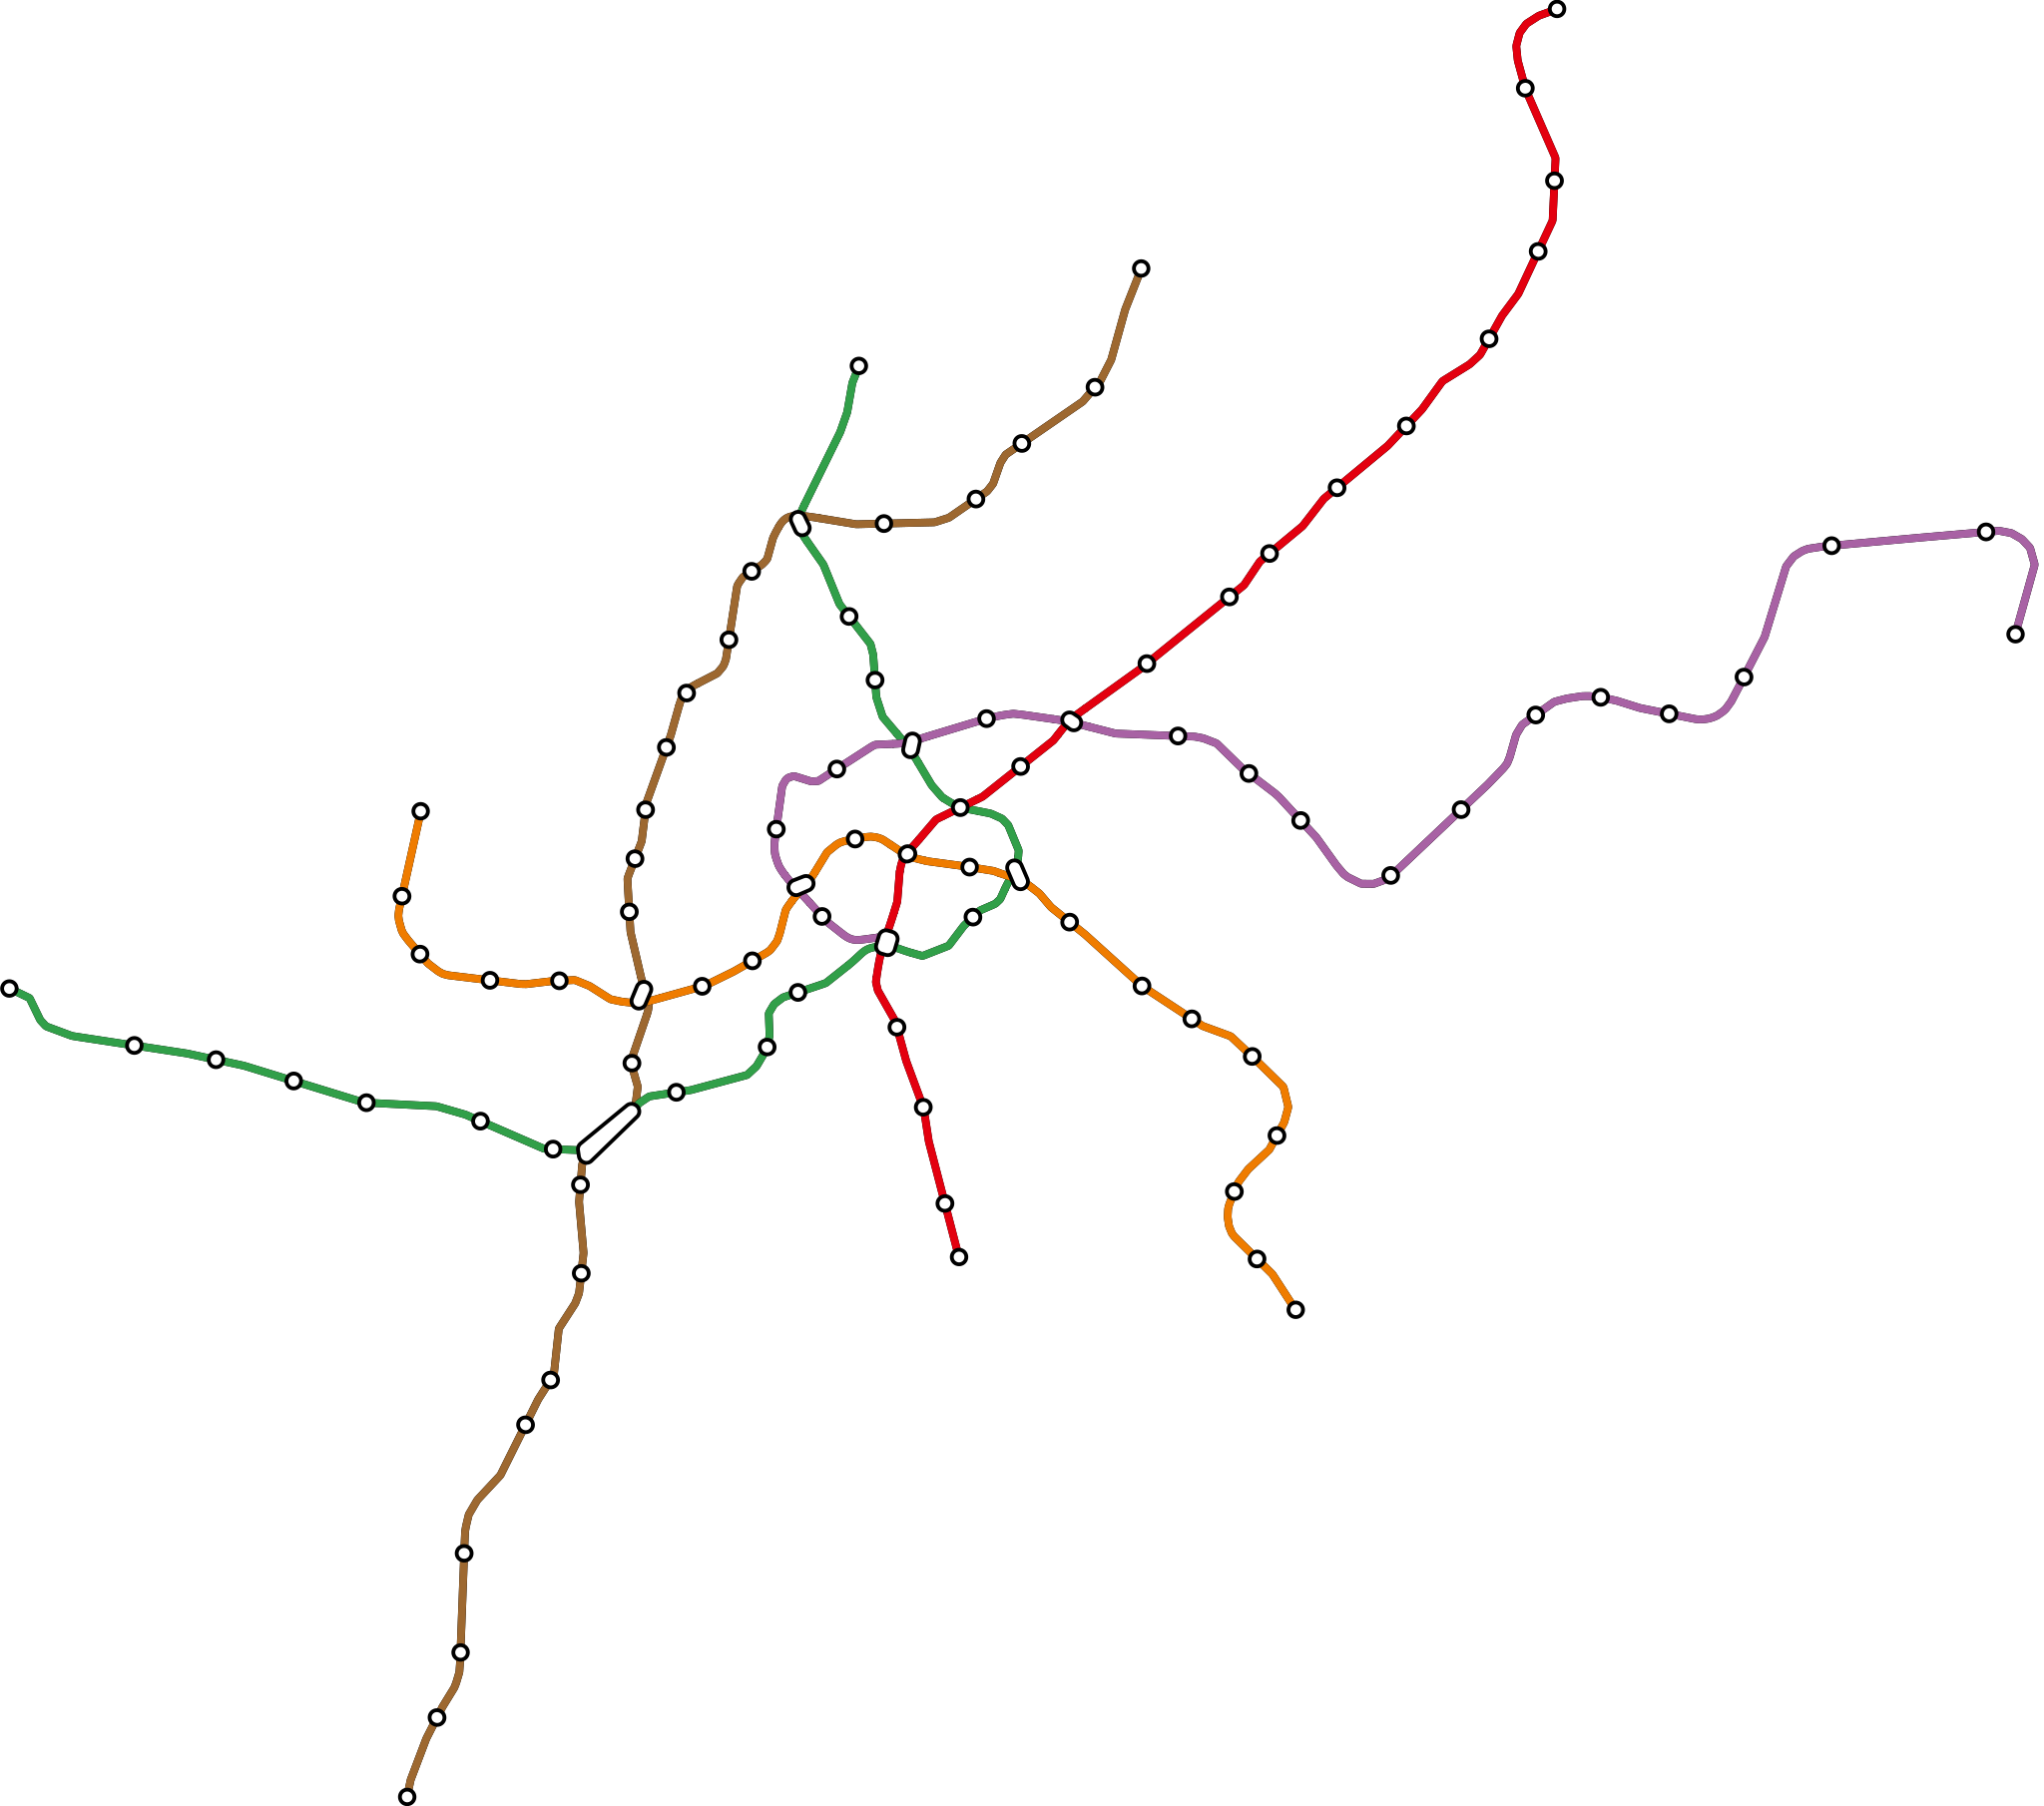
\includegraphics[width=0.414\textwidth]{figures/octi_input.pdf}
	\hspace{1cm}
	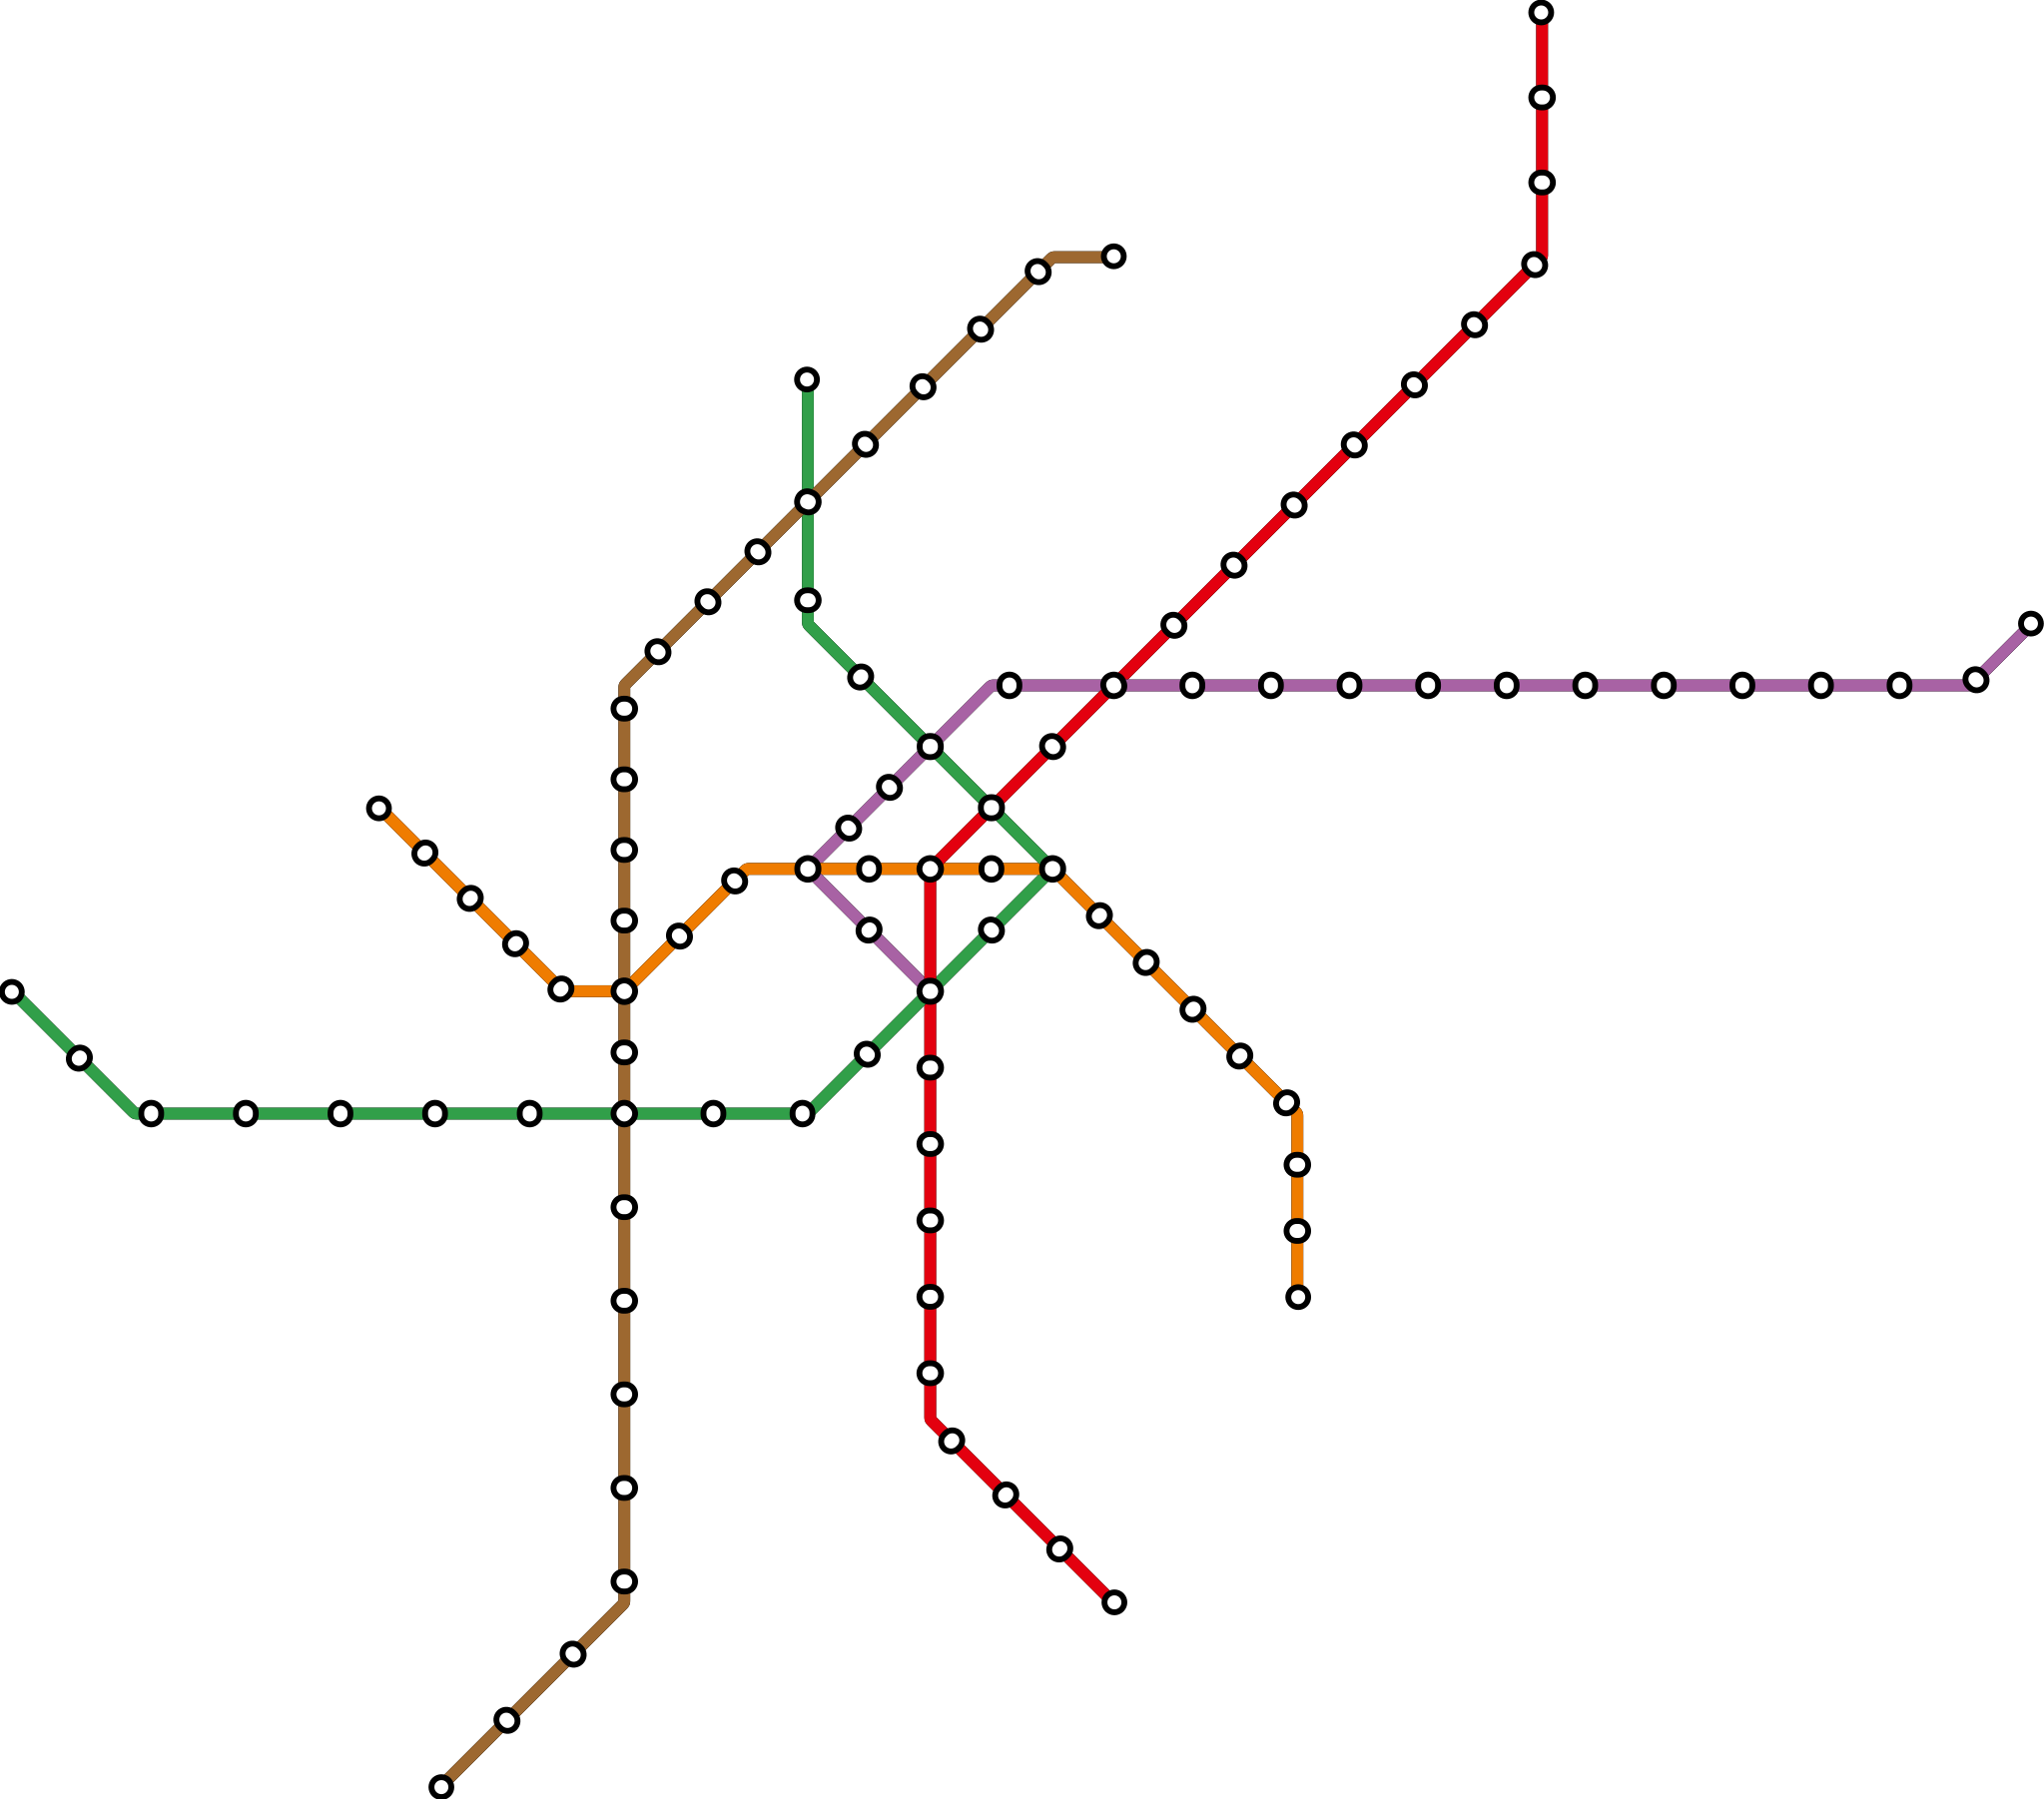
\includegraphics[width=0.414\textwidth]{figures/octi.pdf}
	\caption{Left: the subway network of Vienna, drawn with real-world geographical station positions and line courses. Right: octilinear drawing rendered with our approximative approach. Schematization took around $0.5 s$. \TODO{update}}
	\label{FIG:examplewien}
\end{figure*}

\TODO{Write intro}

Basic approach:

\begin{enumerate}
	\item Input: line graph $\iG = (\iV, \iE, L)$.
	\item Build a $X\times Y$ grid graph $\gG$ whose bounding box matches that of the input line graph.
	\item Add special bend edges which penalize line bends along paths in $\gG$.
	\item For each edge $\{u, v\}$ in the line graph, find grid node pairs $\psi(u)$ and $\psi(v)$ and non-overlapping and non-crossing paths between those pairs such that the sum of the following objectives is minimized: (1) the distance between the geographical position of $u$ and the (pseudo-) geographical position of $\psi(u)$, (2) the path costs between grid node pairs, (3) the line bend costs at grid node pairs. This is strongly related to the (both NP-hard) $k$-Disjoint Paths Problem (DPP) and the Subgraph Homeomorphism Problem (SHP)).
	\item Optimization can be done exactly via an ILP, or with an efficient approximation algorithm which first defines an order on the input line edges, greedily routes the edges in this order on the grid graph iteratively, and optimizes this initial drawing with a local search approach afterwards.
\end{enumerate}

\subsection{Problem definition}

Given an undirected labeled input graph $\iG = (\iV, \iE, L)$, where $\iV$ are stations, $\iE$ are connections between those stations and each edge $\ie \in \iE$ is labelled with a subset $L(e) \in \mathcal{L}$ of lines travelling on this edge.
We call $\iG$ the $\emph{line graph}$.
We say $\drawing{\iG} = (\drawingpossym, \drawingcurvesym)$ is a drawing of $\iG$, where $\drawingpos{\iv}$ assigns a position to every node $\iv \in \iV$ and $\drawingcurve{\ie} = (q_0, q_1, \dots, q_n)$ assigns a piecewise linear curve to every edge $\ie \in \iE$.
The initial input drawing $\initdrawing{\iG}$ assigns each node a geographical real-world position.
Optionally, each edge an may be assigned its real-world course.
Our goal is to find a schematic drawing $\mathcal{D}'_G$ that resembles a classic Metro Map.
This is usually formalized as a set of hard and soft constraints \cite{noll05, noll11}.
The hard constraints may be summarized as:
%
\begin{enumerate}
\setlength\itemsep{.1em}
\item \emph{Octilinearity}. Each edge curve $\drawingcurve{\ie}$ may only consist of segments whose orientation is a multiple of $45^{\circ}$.
\item \emph{Topology Preservation}. The topology of the line graph should be respected. No crossings between edges should be introduced, non-incident edges should never share common points and the circular ordering of edges around adjacent nodes should be preserved.
\end{enumerate}
%
Additionally, the following soft constraints are usually employed:
%
\begin{enumerate}
\setlength\itemsep{.1em}
\item \emph{Edge Monotony}. The number of edge bends should be minimized and large angles preferred.
\item \emph{Edge Length}. The length of the edge curves should be minimized.
\item \emph{Map Density}. There should be a minimum distance $\gmind$ between the anchor points of curves to ensure readability.
\item \emph{Geographical Accuracy}. The original node positions should be changed as little as possible.
\end{enumerate}
%
Soft constraint 4 (Geographical Accuracy) is usually weakened to only apply to nodes with a degree different than 2 (intersection nodes and terminus nodes), as this both improves the overall map appearance and simplifies the problem.
The same is done in this work.

Previous work defined the problem as finding an octilinear \emph{embedding} of the input graph, i.e. each edge is represented by a straight octilinear arc.
We are interested in octilinear \emph{drawings} and therefore use a slightly different approach.
We state the problem as finding the optimal posititions $\drawingpos{\iv} \in \mathbb{N}^2$ on a grid for each station node and curves $\drawingcurve{\ie} = (q_0, q_1, \dots, q_n)$, $q_i \in \mathbb{N}^2$ connecting them. 
Most importantly, for two succeeding points $q_i = (x_i, y_i)$ and $q_{i+1} = (x_{i+1}, y_{i+1})$, we require their Chebyshev distance $D_\text{Ch}(q_i, q_{i+1}) = \max \{|x_{i+1} - x_i|, |y_{i+1} - y_i|\}$ to be exactly 1, which ensures octilinearity of the final drawing.

To project this grid onto a map plane, we use a scale factor $\gScale$, which is essentially the height and length of a grid cell.
If $\gScale$ is set to $\gmind$, a minimum distance between any two grid points is guaranteed to be greater or equal to $\gmind$.
We choose the dimensions $X\times Y$ of the grid in such a way that it matches the bounding box of the input line graph.

\subsection{Related Work}

\TODO{todo}

\section{Octilinear Grid Graph}
\label{SEC:gridgraph}

We use an auxiliary undirected grid graph $\gG = (\gV, \gE)$ with diagonal edges (Fig.~\ref{FIG:grids}, left).
For every position $(x, y)$ on a $X\times Y$ grid, we add a grid node $\ggv{x}{y}$.
Each grid node $\ggv{x}{y}$ is connected with its 8 direct neighbors (except at the grid boundaries) $N^0(\ggv{x}{y}), \dots, N^7(\ggv{x}{y})$, where $N^0(\ggv{x}{y})$ is the ``north'' neighbor of $\ggv{x}{y}$, $N^1(\ggv{x}{y})$ the ``north-east'' neighbor, etc..
Each path $\gPath = (\gv_0, \gv_1, \dots, \gv_n), \gv_i \in \gV$ now represents an octilinear curve with cost $\gPcost{\gPath} = (n - 1) \cdot \gHopcost$, where $\gHopcost$ is the ``hop'' cost of using a single grid edge.

\subsection{Penalizing Line Bends}

To later be able to optimize soft constraint (1) between stations, we additionally want the total cost for a path in $\Gamma$ to reflect the number and accuteness of bends.
The penalty for a bend should be weighted by its degree - either $135^{\circ}$, $90^{\circ}$ or $45^{\circ}$.
We call these penalties $\gPturn{135}$, $\gPturn{90}$ and $\gPturn{45}$.
A straight pass through a node should go unpunished, so $\gPturn{180} = 0$.
Since we aim for a ``smooth'' path through $\gG$ and want to favor obtuse angles, we require $\gPturn{180} \leq \gPturn{135} \leq \gPturn{90} \leq \gPturn{45}$.

We extend our cost function and now want to search for the path $\gPath = (\gv_0, \gv_1, \dots, \gv_i, \dots, \gv_n)$ which minimizes
\begin{align}
	\gPcost{\gPath} = (n - 1) \cdot \gHopcost + \sum_{i=1}^{n - 1} t(\gv_{i-1}, \gv_{i+1}),
\end{align}
where $t(\gv_{i-1}, \gv_{i+1})$ is the angular bend cost between edges $\{\gv_{i-1}, \gv_{i}\}$ and $\{\gv_{i}, \gv_{i+1}\}$, that is, either 0, $\gPturn{135}$, $\gPturn{90}$ or $\gPturn{45}$.

\begin{figure}
  \centering
	$\vcenter{\hbox{\includegraphics[width=0.474\textwidth]{figures/grid.pdf}}}$
	\caption{Left: A shortest path between $t$ and $u$ on a grid graph with uniform edge cost. Path bends are not minimized. Right: Two shortest path between $(t, u)$, and $(v, w)$ on our octilinear grid graph with uniform grid edge cost $1$ and additional path bend penalties $\gPturn{135} = 1$, $\gPturn{90} = 1.5$ and $\gPturn{45} = 2$. Path $(t, u)$ acts as an obstacle for $(v, w)$.}
	\label{FIG:grids}
\end{figure}

We model this by adding 8 auxiliary port nodes $\gpv{x}{y}{0}, \dots, \gpv{x}{y}{7}$ to every grid node (Fig.~\ref{FIG:gridgraph}).
Each port again corresponds to an outgoing angle in clockwise fashion and is connected to $\ggv{x}{y}$ via sink edges $\gse{x}{y}{0}, \dots, \gse{x}{y}{7}$.
These sink edges allow us to leave from and arrive at an original grid node $\ggv{x}{y}$.
For paths passing through $\ggv{x}{y}$, we connect each port $\gpv{x}{y}{i}$ with its 7 - i succeeding (in clockwise fashion) sibling ports at position $j$ with bend edges $\gbe{x}{y}{i}{j}$, $\gbe{x}{y}{i}{j}$, and so forth.

\begin{figure}
  \centering
	$\vcenter{\hbox{\includegraphics[width=0.45\textwidth]{figures/node.pdf}}}$
	\caption{A $5\times3$ octilinear grid graph. Each node $\ggv{x}{y}$ has 8 ports $\gpv{x}{y}{0}, \dots, \gpv{x}{y}{7}$ which are connected to $\ggv{x}{y}$ by direct sink edge $\gse{x}{y}{0}, \dots, \gse{x}{y}{7}$. Each port is additionally connected to its $180^{\circ}$, $135^{\circ}$, $90^{\circ}$ and $45^{\circ}$ neighbor ports by bend edges $\gbe{x}{y}{i}{j}$.}
	\label{FIG:gridgraph}
\end{figure}

To be able to distinguish the different node and edge types, we define the set of original grid nodes as $\gV^g \ni \ggv{x}{y}$, the set of port nodes as $\gV^p \ni \gpv{x}{y}{i}$, the set of bend edges as $\gE^b \ni \gbe{x}{y}{i}{j}$, the set of sink edges as $\gE^s \ni \gse{x}{y}{i}$ and the set of original grid edges as $\gE^g$.
Note that $\gV = \gV^g \cup \gV^p$ and $\gE = \gE^t \cup \gE^s \cup \gE^g$.

Additionally, for each $\gv \in \gV$, we define $\gv^* \in \gV^g$ to be the original grid node belonging to $\gv$ (this may be $\gv$ itself).
For ease of notation, we denote by $P(\gv)$ the grid coordinates of the original grid node $\gv^* = \ggv{x}{y}$ belonging to $\gv$.

As we want to prevent the use of sink edges in pass-through nodes, we set a uniform sink edge cost $\gSinkcost$ high enough so that a sink edge is always more expensive than a bend edge, for example $\gSinkcost = \gPturn{45}$
In a shortest path from $s$ to $t$, the only sink edges are then a leaving sink edge adjacent to $s$ and an arriving sink edge adjacent to $t$.

\subsection{Modelling Edge Costs}

\begin{figure}
  \centering
	$\vcenter{\hbox{\includegraphics[width=0.454\textwidth]{figures/path.pdf}}}$
	\caption{Two octilinear grid graphs and the same path $(\ggv{1}{0}, \ggv{1}{1}, \ggv{0}{2})$ on them. Right: without explicit bend edges for penalizing bends. Left: with explicit bend edges and port nodes. Each grid node is now represented by two nodes: for the start and end node, the original grid node and a leaving port edge. For pass-through nodes ($\ggv{1}{1}$), an arriving and a leaving port node with an edge corresponding to the bend at the grid node between.}
	\label{FIG:path}
\end{figure}
\begin{figure}
  \centering
	$\vcenter{\hbox{\includegraphics[width=0.48\textwidth]{figures/paths.pdf}}}$
	\caption{1. A $180^{\circ}$ pass through a node $\gv$. 2. A $90^{\circ}$ pass through $\psi$. 3. A $45^{\circ}$ pass through $\gv$ simulated by a $180^{\circ}$ and $135^{\circ}$ pass. 4. A $90^{\circ}$ pass through $\gv$ simulated by two $135^{\circ}$ passes. }
	\label{FIG:paths}
\end{figure}
%
As both a $45^{\circ}$ port edge and a $90^{\circ}$ port edge may be substituted by cheaper edges, special care has to be applied to the modelling of the actual edge costs.
For example, a $45^{\circ}$ bend can be simulated by first passing $\ggv{x}{y}$ on a $180^{\circ}$ port edge, and then again on a $135^{\circ}$ port edge (Fig.~\ref{FIG:paths}.3).
As we only require $\gPturn{180} \leq \gPturn{135} \leq \gPturn{45}$, this path may be cheaper than $\gPturn{45}$, undermining our penalty system. 
Similarily, a $90^{\circ}$ degree bend can be simulated by two cheaper $135^{\circ}$ port edges (Fig.~\ref{FIG:paths}.4).

To prevent the shortcuts described above, we first introduce a constant $a \geq 0$ and offset the bend costs by $a$.
We call these updated port edge costs $\gPturnEdge{180}, \dots, \gPturnEdge{45}$ and choose $a$ in a way such that the following inequalities are fullfilled:
%
\begin{align}
	2a + 2\gPturn{135} &\geq a + \gPturn{90} \label{CONSTRS:sim90}\\
	2a + \gPturn{135} + \gPturn{90} &\geq a + \gPturn{45}\label{CONSTRS:sim45}.
\end{align}
Ineq.~(\ref{CONSTRS:sim90}) ensures that simulating a $90^{\circ}$ bend with two $135^{\circ}$ passes is never cheaper than $\gPturnEdge{90}$.
Ineq.~(\ref{CONSTRS:sim45}) ensures that simulating a $45^{\circ}$ bend with a $135^{\circ}$ pass and a $180^{\circ}$ pass is never cheaper than $\gPturnEdge{45}$.

The inequalities are fullfilled for $a = \gPturn{45} - \gPturn{135}$.

The shortest path $\gPathOcti$ from an original grid node $s = \gv_0$ to another original grid node $t=\gv_{n'}$ on our octilinear grid graph with bend penalties will now consist of \emph{two} nodes for each original grid node: for the start and end node, the original grid node and a single port node appear in the path (Fig.~\ref{ref:path}).
For pass-through nodes, a port node for arriving at and a port node for leaving the original grid node appears (w.l.o.g., we ignore the case where a bend edge is replaced by two bend edges with similar cost, as this does neither affect the final path on the grid graph, nor the cost of that path).

This shortest path $\gPathOcti = (\gv_0, \gv_1, \dots, \gv_{n'})$ thus always describes a path $\gPath = (\gv^*_0, \gv^*_2, \gv^*_4, \dots, \gv^*_{n})$ on the corresponding original grid graph \emph{without} bend penalties, with $|p| = n = |p'| / 2 = n' / 2$ and has the cost
%
\begin{align}
	\gPcostOcti{\gPathOcti} = \overbrace{2 \gSinkcost}^{\makebox[0pt]{$\scriptstyle{\text{sink edges}}$}} + \underbrace{\left(n - 1\right) \cdot \gHopcost}_{\makebox[0pt]{$\scriptstyle{\text{grid hops}}$}} + \overbrace{\sum_{i=1}^{n - 1} a + t\left(\gv^*_{2i - 2}, \gv^*_{2i+2}\right)}^{\makebox[0pt]{$\scriptstyle{\text{offsetted bend costs}}$}}\label{EQ:cost}.
\end{align}
%
To get rid of the constant offset $a$, we set $c_{135} = 1$, $c_{90} = 1.5$ and $c_{45} = 2$, which means $a = 1$.
If we then set the cost of a single grid edge $\gHopcost = 1 = a$ and the actual grid edge costs to $\gHopcostOcti = \gHopcost - a = 0$, we can rewrite Eq.~\ref{EQ:cost} as  
%
\begin{align}
	\gPcostOcti{\gPathOcti} &= 2 c_s +  \left(n - 1\right) \cdot \gHopcostOcti + \sum_{i=1}^{n - 1} \gHopcost + t\left(\gv^*_{2i - 2}, \gv^*_{2i+2}\right) \\
	     &= 2 c_s + \left(n - 2\right) \cdot \gHopcost + \sum_{i=1}^{n - 1} t \left(\gv^*_{2i - 2}, \gv^*_{2i+2}\right) \\
	     &= 2 c_s + \gPcost{\gPath} - \gHopcost = \gPcost{\gPath} + 2 \gSinkcost - 1.
\end{align}
%
As the shortest path $p'$ thus minimizes $c(p) + 2 \gSinkcost - 1$, it also minimizes $\gPcost{\gPath}$.

\section{Optimal Solution via ILP}

Using the octilinear grid graph, we now define the problem of finding the optimal metro-map drawing on the grid defined by $\gG$ like this: find grid nodes for each input node and non-intersecting shortest paths in the grid graph between the grid nodes for adjacent input nodes.
The ordering of paths at grid node candidates should match the original embedding.
%The shortest paths in the grid than form an octilinear drawing of $\gG$ in which the original embedding is preserved.
This solution should minimizes the sum of (1) all path costs, (2) the distance between the original and the grid position of a station node with a degree different than 2, and (3) the line bend penalties at stations (which are not covered by the path costs on $\gG$).

We first describe how to solve this problem exactly using an Integer Linear Program (ILP).
To encode the direction of a path from $\gv_s$ to $\gv_t$ in the ILP, we first model each undirected grid edge $\{\gv, \gv'\}$ as a pair of directed edges $(\gv, \gv')$ and $(\gv', \gv)$.
%This transforms our undirected grid graph into an equivalent directed grid graph.
%To get unique start and end nodes for the shortest path calculations, we also treat each input edge $\ie = \{s, t\}$ now as a directed edge $(s, t)$.
%As the shortest paths in $\gG$ are symmetric, it does not matter whether we chose $\ie = (s, t)$ or $\ie = (t, s)$.

To be able to later retrieve the placement of stations, we add binary decision variables $\gvused{\iv}{\gv}$ for each input node $\iv$ and grid node $\gv \in \gV^g$ which should be 1 of $\iv$ was assigned to $\gv$, or 0 otherwise.
We denote this grid node as $\gv_\iv$.
If $\deg(\iv) \neq 2$, $\gvused{\iv}{\gv}$ is added to the objective function with the distance between the original position of $\iv$ and the position induced by $\gv$ as a coefficient.
To be able to deduce the course of the shortest paths, we define binary variables $\geused{\ie}{\ge}$ for each input edge $\ie$ and each grid edge $\ge$ which should be 1 if $\ge$ is used in path for $e$, or 0 otherwise.
$\geused{\ie}{\ge}$ is added to the objective function with the cost of grid edge $\ge$ as a coefficient.

\subsection{Station Placement}

To ensure that each input node $\iv \in \iV$ is assigned to exactly one grid node $\ggv{x}{y} \in \gV^g$, we add the following constraint:
%
\begin{equation}
  \forall \iv \in \iV: \sum_{\gv \in \gV^g} \gvused{\iv}{\gv} = 1. \label{EQ:onegvperiv}
\end{equation}
%
As a grid node can either be assigned a single input station, used as a pass-through for a single input edge, or be not used at all, we additionally add the following constraint:
%
\begin{equation}
  \forall \gv \in \gV^g: \sum_{\iv \in \iV} \gvused{\iv}{\gv} + \sum_{\ie \in \iE} \sum_{\ge \in \gE^b_\gv} \geused{\ie}{\ge} \geq 1, \label{EQ:singleuse}
\end{equation}
%
where $\gE^b_\gv$ is the set of bend edges adjacent to $\psi$. 
If an input station is assigned to $\gv$, the first sum is already 1, forbidding further use.
Similarily, if $\gv$ is used as a pass-through, it cannot be assigned to an input station node or be used as a pass-through by another path.
Note that Equation~\ref{EQ:singleuse} also enforces that a grid edge $\ge$ can only be used by a single path, as a second path using $\ge$ would have to either arrive or pass through a grid node that is already used by the other path on $\ge$.

\subsection{Edge Continuity}

To globally compute the optimal paths on $\gG$ between all adjacent input nodes, we build on the standard formulation of the shortest path problem as a Linear Program.
We first have to make sure that edges assigned to the path from $\gv_s$ to $\gv_t$ are connected.
We add the following constraints (where $e = \{s, t\}$):
%
\newcommand\Psum[1]{\sum_{\makebox[0pt]{$\scriptstyle#1$}}}
%
\begin{align}
	&\forall \ie \in \iE\ \forall \gv \in \gV^p:& \Psum{\ge \in \text{out}(\gv)} \geused{\ie}{\ge} - \Psum{\ge \in \text{in}(\gv)} \geused{\ie}{\ge}& = 0, \label{EQ:cont_port} \\
	&\forall \ie \in \iE\ \forall \gv \in \gV^g:& x_{t\psi} - 2x_{s\psi} + \Psum{\ge \in \text{out}(\gv)} 2\geused{\ie}{\ge} - &\Psum{\ge \in \text{in}(\gv)} \geused{\ie}{\ge} = 0. \label{EQ:cont_grid}
\end{align}
%
Equation~\ref{EQ:cont_port} guarantees that the number of outgoing and incoming edges at each port node is the same.
% This ensures a continuous path between $\gv_s$ and $\gv_t$.
%
Equation~\ref{EQ:cont_grid} handles $\gv_s$ and $\gv_t$.
Here we count an outgoing edge twice, which means that the grid node could only make up for an outgoing edge with two incoming edges.
This, however, would mean that our shortest path split somewhere, which is prevented by Equation~\ref{EQ:cont_port}.
The only way to fullfill the constraint is thus for $\gv$ to be the source node $\gv_s$ for the input edge.
Similarily, the only way to counter an incoming edge is for $\gv$ to be the target node $\gv_t$ for the input edge.

\subsection{Preservation of Embedding}

To preserve the input embedding, it is enough to guarantee that no two paths in $\gG$ intersect and that the circular ordering of adjacent edges is the same as in the input graph.
Equation~\ref{EQ:singleuse} already prevents paths crossing at grid nodes.
Because our octilinear grid graph is not planar, we also have to prevent crossings at intersecting grid edges.
We define $\gE^d$ as the set of diagonal grid edges and say that for $\ge \in \gE^d$, $\ge^{\times} \in \gE^d$ is the diagonal edge crossing $\ge$. 
We then add the following constraint:
%
\begin{equation}
  \forall \ge \in \gE^d: \Psum{\ie \in \iE} \geused{\ie}{\ge} + \geused{\ie}{\ge^{\times}} \leq 1. \label{EQ:crossing}
\end{equation}
%
To ensure that the edge ordering at nodes remains the same, we would first like to have a variable $\dir{\iv}{\ie} \in \{0, \dots, 7\}$ which tells us the direction of input edge $\ie$ at adjacent input node $\iv$ in the final octilinear drawing.
To get the desired assignments, we add the following constraints:
%
\begin{align}
  \forall \ie = \{s, t\} \in \gE&: \sum_{\gv \in \gV^g} \sum_{p = 1}^7 p \geused{\ie}{(\psi,  \psi^p)} - \dir{s}{e} = 0\label{EQ:dirfrom} \\
  \forall \ie = \{s, t\} \in \gE&: \sum_{\gv \in \gV^g} \sum_{p = 1}^7 p \geused{\ie}{(\psi^p, \psi)} - \dir{t}{e} = 0\label{EQ:dirto}
\end{align}
%
In Equation~\ref{EQ:dirfrom}, each outgoing sink edge $(\gv,  \gv^{p}), p \in {0, \dots, 7}$ adds $p$ to the sum.
As Equations~\ref{EQ:cont_grid} and \ref{EQ:singleuse} ensures that only a single outgoing sink edge in the grid graph may be used by the path for an input edge, we can be sure that the left side of the equation always exactly equals the octilinear direction $0, \dots, 7$ of $e = (s, t)$ at $s$.
The only way to fullfil the constraint is thus to set the value of $\dir{s}{e}$ to the octilinear direction.
Equation~\ref{EQ:dirfrom} is modelled equivalently for paths incoming at $t$.

To finally preserve the circular edge ordering, we apply a trick originally used in \cite{noellenburg}.
If $v_0, \dots, v_p, \dots, v_{\text{deg}(u) - 1}$ is the clockwise ordering of nodes adjacent to u in the original embedding, then $\dir{v}{(v, u_{p})} < \dir{v}{(v, u_{p + 1})}$ has to be true for all but one $p \in \{0, \dots, \text{deg}(u) - 1\}$ in the final octilinear drawing.
This can be enforced with the following constraints, which we add for all  $u \in \iV$ with $\deg(u) > 2$:
%
\begin{align}
  \dir{v}{(v, u_{p + 1})} - \dir{v}{(v, u_{p})} + 8\cdot\beta_p(v) &\geq 1,\label{EQ:dirs}\\
  \sum_{p = 0}^{\deg(u)-1} \beta_p(v) &\geq 1\label{EQ:onedef}.
\end{align}
%
If $\dir{v}{(v, u_{p})} \not< \dir{v}{(v, u_{p + 1})}$, then $\dir{v}{(v, u_{p + 1})} - \dir{v}{(v, u_{p})} \leq 0$ and the only way to fullfill Equation~\ref{EQ:dirs} is to set $\beta_p(v)$ to 1.
Equation~\ref{EQ:onedef} ensures that this can only happen once.

\subsection{Avoiding Line Bends}

So far, our shortest paths only penalize line bends along paths.
We have to ensure that line bends at input nodes are equivalently penalized.
We would like to have binary variables telling us whether edges $e$ and $f$ in the input graph describe a $45^{\circ}$, $90^{\circ}$, $135^{\circ}$ or $180^{\circ}$ bend at their joint node in the final drawing.
%As $G$ is not a multigraph, this joint node is unique.

We first note that for two directional variables $\dir{u}{e}$ and $\dir{u}{f}$, $\dir{u}{e} - \dir{u}{f} \mod 8$ is either 1 or 7 for $45^\circ$ bends, 2 or 6 for $90^\circ$ bends, 3 or 5 for $135^\circ$ bends and 4 for $180^\circ$ bends.
As modulo cannot be used directly in an ILP, we use the following equivalent constraint for each pair $e, f$ of edges in the input graph adjacent at node $u$ and sharing a line:
%
\begin{equation} 
  0 \leq \dir{u}{e} - \dir{u}{f} + 8 \gamma_{ef} \leq 7 \label{EQ:dirneg}.
\end{equation}
%
%The auxiliary binary variable $\gamma_{ef}$ will be 1 if $\dir{u}{f} > \dir{u}{e}$.
%As both $\dir{u}{e}$ and $\dir{u}{f}$ are in the range $[1, 8]$ and as $\dir{u}{e} \neq \dir{u}{f}$ (per Eq.~\ref{EQ:singleuse})
We then have $\dir{u}{e} - \dir{u}{f} + 8 \gamma_{ef} = \dir{u}{e} - \dir{u}{f} \mod 8$, which we will denote by $\dirdiff{e}{f}$.
We now add binary decision variables $\bend{e}{f}{0}, \dots, \bend{e}{f}{7}$ for each of the 8 possible values of $\dirdiff{e}{f}$ and the following constraint for each pair of adjacent input edges:
%
\begin{equation} 
  \dirdiff{e}{f} - \sum_{i = 0}^7 i\bend{e}{f}{i} = 0 \label{EQ:bendassign}.
\end{equation}
%
To make sure that only one of the bend variables is set to 1, we add the following constraint:
%
\begin{equation} 
  \sum_{i = 0}^7 \bend{e}{f}{i} = 1 \label{EQ:bendsum}.
\end{equation}
%
Each of the 8 bend variables is then added to the objective function with its corresponding penalty.

\subsection{ILP Complexity}

For an $X \times Y$ grid, our octilinear grid graph has $\Theta(XY)$ edges and nodes.
For the station placement, we need ${\Theta}(|V|XY)$ variables.
Additionally, Equations~\ref{EQ:onegvperiv} and \ref{EQ:singleuse} add ${\Theta}(|V|XY)$ constraints.
For the shortest path calculations, we need ${\Theta}(|E|XY)$ variables and constraints.
For the preservement of the embedding, Equation~\ref{EQ:crossing} adds ${\Theta}(XY)$ constraints.
Equations~\ref{EQ:dirfrom} and \ref{EQ:dirto} add ${\Theta}(|E|)$ constraints.
Equations~\ref{EQ:dirs} and \ref{EQ:onedef} add ${\Theta}(|V|)$ constraints.
Finally, for avoiding line bends and input nodes, we add at most number of $8\times7$ auxiliary variables per input node (as there can be at most $8\times7$ edge pairings per input node in our octilinear setting) and at most $8^2\times7$ bend variables per input node.
Similarily, Equations~\ref{EQ:dirneg}, \ref{EQ:bendassign} and \ref{EQ:bendsum} all add at most $8\times7$ constraints per input node, so the overall number of constraints and variables for the line bend penalty at input nodes is ${\Theta}(|V|)$.
The total number of constraints and variables in our ILP is thus ${\Theta}(|E|XY + |V|XY) = \mathcal{O}(|E|XY)$.

\section{Approximative Solution}

ILP solution times tend to get very big for complex input graphs. \TODO{how big?}
This section describes a fast method to solve the problem approximatively.
Our method works as follows:
  (1) Contract all nodes of degree 2.
  (2) Order the remaining edges of the input graph.
  (3) For each (ordered) input edge $e = \{u, v\}$, calculate the shortest path from a set of possible start nodes $S$ to a set of possible target nodes $T$ on the grid graph. If the grid node for $u$ or $v$ has already been settled, the corresponding node set has size 1. Paths already calculated act as obstacles.
  (4) If no initial drawing could be found, randomize the ordering and try again.
  (5) Optimize the initial drawing via a local search approach where individual nodes are moved to one of their 8 neighboring positions and adjacent edges re-routed.
  (6) Re-insert the contracted degree 2 nodes into the corresponding edge curves equidistantly.

Each step is described in detail in this section.
We additionally explain how the shortest path search on the grid graph can be sped up with an $A^*$ heuristic.

\subsection{Input Edge Ordering}
%
\begin{figure}
  \centering
	\includegraphics[width=0.219\textwidth]{figures/node_order.pdf}
	\hfill
	\includegraphics[width=0.229\textwidth]{figures/partial_drawn.pdf}
	\vspace{-.3cm}
	\caption{Left: Input line graph with edge processing order. Right: Line graph routed on grid after step 6.}
	\label{FIG:order}
\end{figure}
%
In addition to the standard degree $\deg(\iv)$ of an input node $\iv$, we define the line degree $\ldeg(\iv)$ of a node to be the number of (non-unique) lines on each adjacent edge.
We then build our initial input edge ordering $(e_0, e_1, \dots, e_{|E|})$ as follows:
  (1) Mark all input nodes as unprocessed.
  (2) Take the unprocessed node $\iv$ with highest line degree $\ldeg(\iv)$ and mark it as dangling.
  (3) As long as there are dangling nodes, take the dangling node $\iv_d$ with highest line degree and add all adjacent edges $\{\iv_d, u_0\}, \dots, \{\iv_d, u_k\}$ leading to an unprocessed node $u_i$ to the edge ordering, where the $u_i$ are sorted in ascending order w.r.t $\ldeg(u_i)$. Mark each $u_i$ as dangling, and $\iv_d$ as processed. 
  (4) If there are no dangling nodes anymore, but unprocessed nodes remain, then the input graph was disconnected. In this case, we start again at (2).
Figure~\ref{FIG:order} gives an example.

\subsection{Edge Routing and Station Placement}
%
\begin{figure}
  \centering
	$\vcenter{\hbox{\includegraphics[width=0.479\textwidth]{figures/heur.pdf}}}$
	\vspace{-.3cm}
	\caption{Left: routing an edge on the grid graph from grid node candidates $S$ for input node $s$ to grid node candidates $T$ for input node $t$ (both within a distance $\hat{d}$ around $t$ and $s$. The grid nodes depicted as full rectangles constitute the hull of the $S$ and $T$, respectively. Right: routing an edge on the grid graph from an already settled grid node $\psi$ to a set $T$ ot target node candidates.}
	\label{FIG:heur}
\end{figure}
%
With an initial edge ordering at hand, we route each input edge $\ie_i = \{\iv, u\}$ through the octilinear grid graph.
To get unique source and target nodes, we again treat each undirected input edge as a directed edge $\ie_i = (s, t)$.
As the grid nodes for $\iv$ and $u$ may be still unknown, we route between node sets $S$ and $T$.
$S$ consists of candidate grid nodes for $s$, $T$ are candidate grid node for $t$.
As candidates, we use all grid nodes within a threshold distance $\hat d$ \TODO{other symbol for that, also update in figure} around the original position of the input node (Fig.~\ref{FIG:heur}).
If both $s$ are $t$ are not settled yet, it may happen that $S$ and $T$ are not disjoint.
To prevent this, we build a local Voronoi diagram: we first define $ST = S \cup T$ and say that for each $\ggv{x}{y} \in ST$, $\ggv{x}{y}$ is placed in $S'_g$ if it is nearer to $s$ than $t$, or in $T'_g$ otherwise.

To prefer grid nodes as candidates that are near the original position of the input node, we offset the cost of each sink edge adjacent to the candidate grid node with the corresponding distance penalty. \TODO{how exactly is the penalty calculated?}

After that, we calculate the set-to-set shortest path between $S$ and $T$ using a standard implementation of Dijkstra's algorithm.
% (to find the shortest path out of a set of source nodes to a set of target nodes, it is enough to init all $\ggv{x}{y} \in S$ with distance 0 and abort the algorithm as soon as any $\ggv{x}{y} \in T_g$ is reached.)
If $s$ or $t$ were not settled before, they are now settled to the start (and/or end) node of the resulting shortest path.

\subsection{Preservation of Embedding}

To prevent paths crossing each other, we update our octilinear grid graph after each Dijkstra run.
Grid nodes that were used as nodes in the previously found shortest path are both \emph{bend-closed} by setting the cost of each adjacent bend edge to $\infty$ and \emph{sink-closed} by setting the cost of each adjacent sink edge to $\infty$.
This effectively prevents any further path to use any of these previously used nodes.
If a node $\ggv{x}{y}$ was settled as the source or target node for the previously routed edge, it may later be used again as a source (or target) node for another input edge.
We then have to open its sink (but not its bend edges) again.

To prevent paths crossing each other at crossing diagonal edges in the grid graph, we additionally close for each diagonal grid edge used in the previously found path all crossing diagonal grid edges by setting their cost to $\infty$.

\begin{figure}
  \centering
	$\vcenter{\hbox{\includegraphics[width=0.479\textwidth]{figures/topoblock.pdf}}}$
	\caption{Left: Part of an input graph $G$. Edges $e$ and $f$ have a clockwise (green) distance of 1 at $v$, meaning that there are no edges between them in an angular, clockwise ordering. Their counterclockwise distance (blue) ist 2. 
	Center: Paths $p(e)$ and $p(f)$ have already been computed. The red area is now blocked for path $p(e)$. Right: Paths $p(e)$ and $p(g)$ have already been computed, but $p(g)$ is placed in such a way that the original edge ordering cannot be respected anymore. }
	\label{FIG:paths}
\end{figure}

To preserve the circular edge ordering at nodes, we update the costs of adjacent sink edges for the grid node used for $s$, and the grid node used for $t$.
We consider Figure~\ref{FIG:paths}.2.
The rendering order at $v$ is $(e, f, g$), and paths $p(e)$ and $p(f)$ have already been routed.
%The path for $e$ uses the sink edge $\gse{}{}{0}$, the path for $f$ uses sink edge $\gse{}{}{3}$.
To respect the input edge ordering at $v$, we have to make sure that $p(g)$ does not enter or leave $\gv$ in the area marked red.
We achieve this by closing each sink edge $\gse{}{}{p}$ that lies between $\gse{}{}{0}$ prior to routing $g$ by setting its cost to $\infty$ (including the sink edges used by $p(e)$ and $p(f)$) (Fig.~\ref{FIG:paths}.2a).

We now consider Figure~\ref{FIG:paths}.3 and assume the rendering order at $v$ to be $(e, g, f)$.
Paths $p(e)$ and $p(g)$ have already been routed.
However, there is no sink edge left at $\gv$ to route $p(f)$ in such a way that the input edge ordering is preserved.
To prevent dead-ends like this, we make sure that there are always enough sink edges left in both directions of $f$.
For example, the clockwise distance between $e$ and $g$ at $v$ is 2 (Fig.~\ref{FIG:paths}.1).
Their clockwise distance is 1.
If $p(e)$ is already routed (Fig.~\ref{FIG:paths}.3), we now close the sink edges $\gse{}{}{0}$ used by $p(e)$, but also the succeeding (in clockwise direction) sink edge $\gse{}{}{1}$ (Fig.~\ref{FIG:paths}.3a).
This guarantees that any path found for $g$ will now leave one sink edge between $p(e)$ and $p(g)$ open, allowing $p(f)$ to be routed in such a way that the original edge order at $v$ will be preserved.

%Note again that in both of the above cases, $\gv$ has already been settled.
%This means that the costs of all bend edges adjacent to $\gv$ have been set to $\infty$.
%We can thus be sure that our sink edge cost are not circumvented, for example, by a path $p(g)$ using $\gse{}{}{2}$ in Figure~\ref{FIG:paths}.3b, and then using the $45^{\circ}$ bend cost connecting port $\gpv{}{}{2}$ and $\gpv{}{}{1}$.

\subsection{Avoiding Line Bends}

\begin{figure}
  \centering
	$\vcenter{\hbox{\includegraphics[width=0.479\textwidth]{figures/linebend.pdf}}}$
	\caption{(1) part of an input line graph with a node $v$ and three adjacent edges $e, g, f$. (2) $g$ and $f$ have already been drawn on the grid graph, $v$ has been settled at $\psi$. (3) the sink edge costs at $\psi$ prior to routing $e$. As $v$ has been settled at $\psi$, the bend edges at $\psi$ are closed and are not depicted. Already used sink edges (depicted in red) have cost $\infty$. Unused sink edges have costs equal to the bend costs induced by letting $p(e)$ leave in the corresponding direction.}
	\label{FIG:linebends}
\end{figure}

Just as in the ILP formulation, our shortest path calculations so far only optimize line bends along paths.
We have to additionally ensure that line bends at nodes are equivalently penalized.
We handle this similar to the edge ordering constraints in the previous section.
Assume a grid node $\gv$ that was already settled for an input node $\iv$ with adjacent edges (in rendering order) $\ie_0, \dots, \ie_i, \dots, \ie_{\deg(v)}$.
Prior to routing an edge $\ie_i$, we calculate the line bend penalty between every already routed edge $\ie_j$, $j < i$ and $\ie_i$ for each of the possible placements of $\ie_i$ on adjacent sink edges.
The sum of the line bend penalties on each adjacent sink edge is then used as the cost for this sink edge (Fig.~\ref{FIG:linebends}).

\subsection{Complexity}

\TODO{Complexity, should be $|E| \times \text{dijkstra}$}


\subsection{Optimization via Steepest Hill Climbing}

\begin{figure}
  \centering
	$\vcenter{\hbox{\includegraphics[width=0.479\textwidth]{figures/optim.pdf}}}$
	\caption{Optimizing an initial drawing (1) by exploring the local search neighborhood, consisting of the 8 neighboring positions (depicted here for node $\psi$) for each settled grid node. All edges adjacent to the node under investigation are re-routed after it is moved to a neighboring position, and the position which yields the biggest improvement is taken (2, 3). Afterwards, the local search continues.}
	\label{FIG:optim}
\end{figure}

The metro maps rendered by our heuristical approach so far already look acceptable.
To further polish the look of our final maps, we employ a local search approach.
Given an octilinear drawing $\drawing{\iG}^0$ on a grid graph $\gG$, we define the local neighborhood of $\drawing{\iG}^0$ as the set of drawings where exactly one grid node position of an input node $v_m$ is moved to one of the 8 neighboring grid position (if free).
For each neighbor of the current drawing, we remove the shortest paths for each edge adjacent to $v_m$, move $v_m$ to the designated new position, re-route all adjacent edges in clockwise ordering and calculate the overall score of the drawing.
At the end, the best neighbor is taken, and the optimization proceeds from there (Figure~\ref{FIG:optim}).

We note that the set of drawings that are reachable by navigating from neighbor to neighbor is not necessarily the complete set of possible octilinear drawings.
This means that the optimal drawing might not be included in this set and is therefore impossible to find.
There are two reasons for that: 
(1) The shortest paths are not necessarily unique.
There might be two (or more) shortest paths between two input nodes which have equivalent cost, but one of them might act as an obstacle which forces a later edge route to follow an adverse path.
During the exploration of the neighborhood, it will depend largely on the implementation which of two equivalent shortest path is chosen locally, and the optimal placement of a particular path might never be chosen.
(2) The final map score does not only depend on the placement of nodes, but also on the order in which edges are rendered.

\subsection{Optimizing Distances between Degree Two Stations}

As our heuristical approach contracts degree two stations in the input graph prior to finding an octilinear drawing, we have to enforce that the distance between contracted stations is at least $\hat d$ after they have been re-inserted into the final drawing. 
We reformulate hard constraint 4 as a soft constraint which is optimized during the steepest hill climbing.
We consider the octilinear drawing before the re-insertation of the contracted nodes.
For an input edge $e$ with an octilinear curve $c(e)$ built of $l$ grid edges and containing $k$ contracted stations, we define a spring force $F_e = c \cdot (k + 1 - l)$.
This spring is relaxed if the $L^\infty$ (grid edge) length $l$ of $e$ is such that we can insert $k$ stations equidistantly with distance 1. \TODO{figure...}
If $F_{u, v} > 0$ (that is, if the hypothetical spring is compressed), we add the potential energy $E_e = \frac{1}{2} c \cdot (k + 1 - l)^2$ to our objective function.
Note that if we also added $E_e$ for $F_e < 0$, we would optimize for a final drawing where the length of any edge is 1.

\subsection{Speed-up Heuristic}

The octilinear grid graph allows for a simple cost heuristic for the path-finding step.
Given a (set) of target nodes, a cost heuristic $h(\gv)$ gives an estimate of the shortest path cost from $\gv$ to any target node.
It is called \emph{admissible} if it never overestimates the real shortest path cost.

We reconsider Figure~\ref{FIG:heur}.
In the right example, it is obvious that the cost for reaching any grid node candidate (or any of its port nodes) in $T$ from a grid node $\gv$ (or any of its port nodes) outside of $T$ is at least the cost of reaching one of the grid nodes that constitute the hull of the node candidates.

The hull $H_t$ of $T$ is just the set of grid nodes in $T$ adjacent to a grid node not in $T$ and can be efficiently computed in $\mathcal{O}(|T|)$.
It can be build prior to the actual shortest-path calculation.

The shortest path cost (minus the arriving sink edge costs) from a node $\gv$ to any node in the hull $H_t$ would thus already be an admissable heuristic.
To get an efficiently computable estimate for the shortest-path cost from $\gv$ to the hull, we use the fact that to reach a grid node $\ggv{x}{y}$ (or any of its port nodes) from a grid node $\ggv{x'}{y'}$ (or any of its port nodes) we have to pass through at least $D_{\text{Che}}((x', y'), (x, y)) - 1$ grid nodes.

We can thus use the following heuristic:
%
\begin{align}
	h(\gv) &= \min\left\{ \left(D_{\text{Ch}}\left(P(\gv), P(\gv') \right) - 1\right) c'_{180}| \gv' \in H_t \right\}\\
	&= \min\left\{ D_{\text{Ch}}\left(P(\gv), P(\gv') \right) - 1 | \gv' \in H_t \right\},
\end{align}
%
as each shortest path has to take some bend edge at the pass-through nodes and the cost of this bend edge is at least $c'_{180} = 1$.

\section{Evaluation}

\subsection{Penalty Experiments}

\section{Conclusions}

\bibliographystyle{ACM-Reference-Format}
\bibliography{octi}

\end{document}